% Printed books have indexes
\ifxetex
	\makeindex
\fi

\begin{document}
% use chapter boxes only for printed books: uncomment % chapter title formatting. It produces a full page with two rectangles along the edges. No change or adaption necessary (or recommended).
% note that this package is not loaded by default. Uncomment the line in main/main.tex to produce the nice chapter pages. Some warnings will occur because of older packages. 
\pagestyle{scrheadings}

% The next command formats the chapter title.
\providecommand{\chapformat}{}
\renewcommand\chapformat[1]{%
    \parbox{\dimexpr\textwidth-\innerRec-2\innerLineWidth-2\adjustTitleWidth\relax}
        {\centering\chapterTitleFont#1}}
     \titlespacing*%
         {\chapter}
         {\leftMar}
         {\beforeSep}
         {\topSep}
         [0cm]
         %\adjustForBindingMargin
         
\providecommand{\chapterbox}{}
\renewcommand\chapterbox{
 \titleformat{\chapter}[display]
     {\bfseries\filcenter}
     {
      \chapterLeadinFont{\chaptertitlename\  \thechapter}\\[\spaceToRule]
    \rule[2mm]{3cm}{2pt}\\
       [\spaceAfterRule]
     }
     {0pt}
     {
       \begin{tikzpicture}[overlay,remember picture]
       \draw [line width=\outerLineWidth]
           ($ (current page text area.north west) + (\outerRec,-\outerRec) $)
           rectangle
          ($ (current page text area.south east) + (-\outerRec,20pt+\outerRec)
          $);
      \draw [line width=\middleLineWidth]
          ($ (current page text area.north west) + (\middleRec,-\middleRec) $)
          rectangle
          ($ (current page text area.south east) +
           (-\middleRec,20pt+\middleRec) $);
      \draw [line width=\innerLineWidth]
          ($ (current page text area.north west) + (\innerRec,-\innerRec) $)
          rectangle
          ($ (current page text area.south east) + (-\innerRec,20pt+\innerRec)
          $);
    \end{tikzpicture}
   \chapformat}
    {}
}



 and comment out \newcommand{\chapterbox}[1]{} to produce nicer looking chapter pages (but also some warnings due to older packages). 
\ifxetex
	%% chapter title formatting. It produces a full page with two rectangles along the edges. No change or adaption necessary (or recommended).
% note that this package is not loaded by default. Uncomment the line in main/main.tex to produce the nice chapter pages. Some warnings will occur because of older packages. 
\pagestyle{scrheadings}

% The next command formats the chapter title.
\providecommand{\chapformat}{}
\renewcommand\chapformat[1]{%
    \parbox{\dimexpr\textwidth-\innerRec-2\innerLineWidth-2\adjustTitleWidth\relax}
        {\centering\chapterTitleFont#1}}
     \titlespacing*%
         {\chapter}
         {\leftMar}
         {\beforeSep}
         {\topSep}
         [0cm]
         %\adjustForBindingMargin
         
\providecommand{\chapterbox}{}
\renewcommand\chapterbox{
 \titleformat{\chapter}[display]
     {\bfseries\filcenter}
     {
      \chapterLeadinFont{\chaptertitlename\  \thechapter}\\[\spaceToRule]
    \rule[2mm]{3cm}{2pt}\\
       [\spaceAfterRule]
     }
     {0pt}
     {
       \begin{tikzpicture}[overlay,remember picture]
       \draw [line width=\outerLineWidth]
           ($ (current page text area.north west) + (\outerRec,-\outerRec) $)
           rectangle
          ($ (current page text area.south east) + (-\outerRec,20pt+\outerRec)
          $);
      \draw [line width=\middleLineWidth]
          ($ (current page text area.north west) + (\middleRec,-\middleRec) $)
          rectangle
          ($ (current page text area.south east) +
           (-\middleRec,20pt+\middleRec) $);
      \draw [line width=\innerLineWidth]
          ($ (current page text area.north west) + (\innerRec,-\innerRec) $)
          rectangle
          ($ (current page text area.south east) + (-\innerRec,20pt+\innerRec)
          $);
    \end{tikzpicture}
   \chapformat}
    {}
}




	\newcommand{\chapterbox}[1]{}
\else
	\newcommand{\chapterbox}[1]{}
\fi
% ---------- Front matter
\frontmatter

% front matter chapter entries use roman page numbering (i, ii, iii, iv, ...)
\pagenumbering{roman}

% switch to basic chapter design
%  Reset the chapter design to a basic one (no box, just underlined chapter title---used for the back and front matter)

\renewcommand*\chapterheadstartvskip{\vspace*{-3\topskip}} 
\renewcommand*\chapterheadendvskip{
  \vskip-.5\baselineskip
  \noindent
  {\color{gray}\rule{\linewidth}{2pt}}
  \par}
\renewcommand*\chapterformat{}
\renewcommand*{\chapterpagestyle}{empty}

% the additional title with the cover is not needed for ebooks
\ifxetex
	%%%%%%%%%%%%%%%%%%%%%%%%%%%%%%%%%%%%%
% Read the /ReadMeFirst/ReadMeFirst.tex for an introduction. Check out the accompanying book "Better Books with LaTeX" for a discussion of the template and step-by-step instructions. The template was originally created by Clemens Lode, LODE Publishing (www.lode.de), mail@lode.de, 8/17/2018. Feel free to use this template for your book project!
%%%%%%%%%%%%%%%%%%%%%%%%%%%%%%%%%%%%%

\thispagestyle{empty}

% Replace "Replace with your Title" with your book title
% Replace "Replace with your subtitle" with your book subtitle
% Replace "Publishing Company, Location" with your company's name and location 
% Upload a low res jpg and a high res png version of your front cover into the "images" folder
% Replace "bover_highres.png" and "bover.jpg" with your file name

\vspace{3cm}
  \begin{center}
	\bfseries \sffamily \Huge EVALUATION STRATEGY PROJECT AND RUBRIC\par
	\bfseries \LARGE Assessment and Evaluation Workshop Notes and Learner Collatoral Manual\par
~\\
	~\\
	\bfseries \small Produced by Peter Sigurdson\par
	
    \ifxetex
		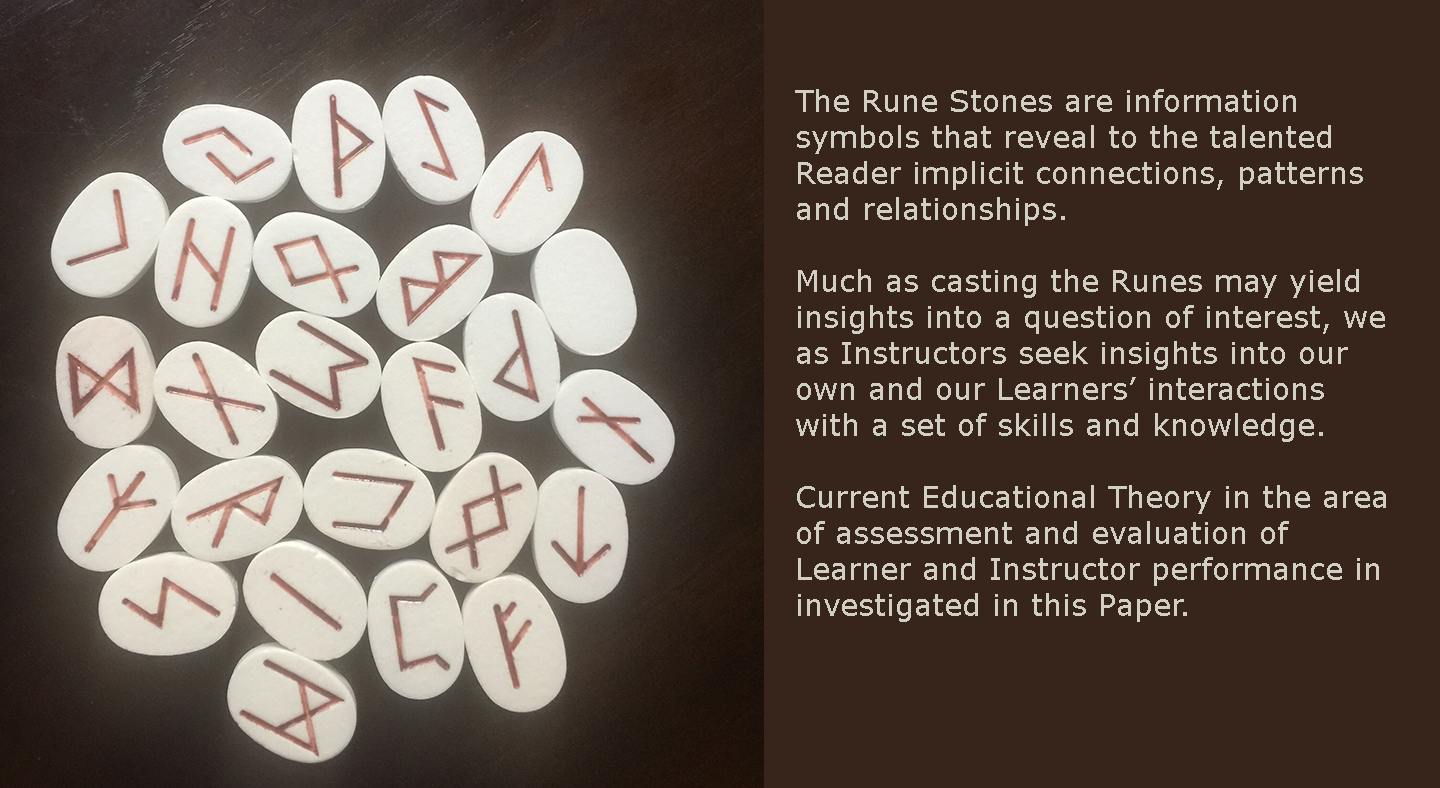
\includegraphics[width=1\textwidth]{images/RuneStones.png}
	\else
    	
\includegraphics{images/cover.jpg}
    \fi
  \end{center}
\newpage
\fi

\begin{chapterpage}{}{p1_foreword:cha}

\begin{myquotation}\large

The absence of data is not the same thing as "No Information"  \newline 
Mr. Spock, Science Officer, First Officer, USS Enterprise

\end{myquotation}
\vspace{2cm}
\begin{myquotation}\large

If you gotta have it explained to you, you ain't never gonna understand it.\newline

Louis Armstrong, American Stage Musician and Performer. Credited with being formative in the development of the Jazz style of music.

\end{myquotation}
\vspace{2cm}
\end{chapterpage}


% surrounding table of contents either with the appropriate style (PDF) or HTML commands (ebook).
\thispagestyle{empty}
\ifx\HCode\undefined 
	% put table of contents on the left side
	\KOMAoptions{open=left}
\else
	\HCode{<nav epub:type="toc">}
\fi

\tableofcontents

\ifx\HCode\undefined
	\KOMAoptions{open=right}
	% finalize page and clear pagestyle to remove header, reset to chapter beginnings on the right side
	\thispagestyle{empty}\pagestyle{empty}\clearpage
\else
	\HCode{</nav>}
\fi
\newpage

% ---------- Main matter
\mainmatter

% reset to normal page numbering (1, 2, 3, ...)
\pagenumbering{arabic}
    
% switch back to basic chapter design
%  Reset the chapter design to a basic one (no box, just underlined chapter title---used for the back and front matter)

\renewcommand*\chapterheadstartvskip{\vspace*{-3\topskip}} 
\renewcommand*\chapterheadendvskip{
  \vskip-.5\baselineskip
  \noindent
  {\color{gray}\rule{\linewidth}{2pt}}
  \par}
\renewcommand*\chapterformat{}
\renewcommand*{\chapterpagestyle}{empty}
% Replace Replace with First Chapter Name
% Replace p1_firstchapter:cha with your chapter title label (no spaces, only lower case letters)
% Replace the text below \end{chapterpage} and insert your own text.

\begin{chapterpage}{ Assessment and Evaluation in Adult Learning}{p1_firstchapter:cha}

\end{chapterpage}
% -------------------- replace or remove text below and paste your own text ------

\section  {Welcome and Introduction}\label{c1_basicformatting:sec}

\begin{itemize}

\item The purpose of this workshop on Assessment and Evaluation in Adult Learning is to enhance your skills as an Instructor in assessing student learning, and to provide the opportunity to experiment with designing evaluation strategies and measures of student learning progress as well as your effectiveness as an Instructor.

\item The evaluation strategies we development will be based on Chapters 3 and 5 of The Art of Evaluation. This textbook is "a practical introduction to learner evaluation in the various contexts of adult education" (Fenwick and Parsons, 2009)

\end{itemize}

\section {Learning Outcomes}

\subsection {Upon completion of this Workshop, the Learner shall be able to describe the operational differences between }

\begin{enumerate}
	\item Diagnostic Evaluations
	\item Formative Evaluations
	\item Summative Evaluations
\end{enumerate}
And be able to identify where in the Learning Content Delivery Cycle each kind of Evaluation should be implemented, what its purpose it, and how the Instructor will utilize the results.

\subsection {Chapter 3: Planning for Evaluation covers the Topics of }

\begin{enumerate}
	\item Why should the Evaluation take place?
	\item What should be evaluated? What do you want the Learners to know?
	\item What do you want to know?
	\item What does the Institution want to know?
	\item What approaches should be used? Here we are factoring in Validity and Reliability.
	\item How much time and resources do you as the Instructor have to do this?
\end{enumerate}

\subsection{Chapter 5 Topics: Choosing an Evaluation Strategy will present the Map of Assessment Methods that are available to us as Instructors:}
The key question here is: What Objective and Subjective strategies should we use to Evaluate Learners' mastery of the Concepts of Chapters 3 and 5? 

How can we best align the methods, instruments and strategies with the learning outcomes?

Are the strategies appropriate for the different types of evaluations? Diagnostic, formative, summative and teaching/training effectiveness.

The Learner shall be able to articulate the differences between Objective and Subjective Evaluations, and categorize the major assessment methods into each bin:
\begin{enumerate}
	\item The Objective Scale evaluators of Multiple Choice, Matching, True/False, and Fill in the Blanks.
    \item The Subjective evaluators of Short Answer, Narrative, and Essay style tests
    \item Student Demonstration of a Skill (Subjective)
    \item Informal student writing: Class Journals, Short Reflection Papers.
\end{enumerate}

\section  {The Toolboxes of Evaluative Methodologies we will be using to assess and evaluate Learning and Instructional Progress:}

\begin{itemize}
\item Include well designed and effective questions
\item Learner Journals
\item Written assignments
\item Performance observation
\item Using Objective Tests
\end{itemize}

\section  {Diagnostic Evaluation:}

Diagnostic evaluation is used to determine student prior knowledge and is generally done at the beginning of a course before theory is presented. 
	Diagnostic evaluation is also a part of the design process done before a course is created. 

For example, data is collected in a "needs assessment" to determine if training is required; and if so, what needs to be taught and what is required of the learner regarding incoming levels of knowledge and experience. 

Diagnostic evaluation of learning occurs in the class/workshop and goes a step further than the design phase of the needs assessment to uncover student expectations of their learning experience.
	Purposes:
		Assess skills, abilities or levels of achievement
		Reveal causes of learning difficulties
		Direct program modification when necessary
	Examples of Assessment for Diagnostic Evaluation:
		Short Essay - The Student Profile (informal)
		Short Essay/Questionnaire - Individual Report Part I in this course (formal)
		Questionnaire/Survey – Needs Assessment sent to participants before a training event or at enrolment (formal)
		Portfolios (formal) (if done before the course begins as in PLAR. See below)
		Verbal & Non-Verbal Q&A, Performance & Observations – Pre-tests, Games, Meet and greet exercise, etc done during the first class or before a new topic is introduced (informal)


Complete the assessment below to determine your prior knowledge before starting the workshop.
Rate items on the scale of Strongly Disagree, Disagree, Agree, and Strongly Agree by placing an ‘X’ in the appropriate box.

\section  {Grading Rubric:}


\section  {References/Citations}
Fenwick, T. and Parsons, J. The Art of Evaluation: A Resource for Educators and Trainers, 2nd Edition. Thompson Educational Publishing, Inc.

\begin{chapterpage}{Peer Review Questions}{p1_secondchapter:cha}

\end{chapterpage}

% -------------------- replace or remove text below and paste your own text ------
\begin{enumerate}
    \item 	Are the methods, instruments and/or strategies aligned with the learning outcomes? Explain.
    \item 	Are the strategies appropriate for the different types of evaluations? Diagnostic, formative, summative and teaching/training effectiveness. Explain.
    \item 	What concerns (if any) do you have with the strategies, methods, content, etc.?
    \item 	Based on what you have learned about creating objective and subjective strategies, what do you think about the objective and subjective strategies created for this evaluation strategy project? What suggestions do you have for improvement?
    \item 	Assess the layout of the evaluation strategies. Are the instructions for the strategies clear and easy to follow? If not, what suggestions do you have for improvement?
    \item 	Do you have any suggestions for different approaches or instruments that can be used for this evaluation strategy project? If so, why? If not, why not?
\end{enumerate}


%%%%%%%%%%%%%%%%%%%%%%%%%%%%%%%%%%%%%
% Read the /ReadMeFirst/ReadMeFirst.tex for an introduction. Check out the accompanying book "Better Books with LaTeX" for a discussion of the template and step-by-step instructions. The template was originally created by Clemens Lode, LODE Publishing (www.lode.de), mail@lode.de, 8/17/2018. Feel free to use this template for your book project!
%%%%%%%%%%%%%%%%%%%%%%%%%%%%%%%%%%%%%


% Command to add some text into the bibliography (between the title and the list of referenced books)
% See https://tex.stackexchange.com/questions/197061/text-between-index-or-bibliography-title-and-content

\bibpreface{Write here the preface of your list of recommended reading titles. Delete this line to have no preface for this section.}

\ifxetex
	\printbibliography
\else
	\newpage
	\bibliographystyle{plainnat}
	\bibliography{bibliography/english}
\fi


\end{document}